%
%-----------------------------------------------------------
%% Computer Music Journal LaTeX template
%%
%% September  2009
%% Author: Cornelia Kreutzer, University of Limerick

%---Document preamble
%
\documentclass[letterpaper, 12pt]{article}

\usepackage{cmjStyle} %use CMJ style
\usepackage{natbib} %natbib package, necessary for customized cmj BibTeX style
\usepackage{graphicx}

\bibpunct{(}{)}{;}{a}{}{,} %adapt style of references in text
\doublespacing
\raggedright % use this to remove spacing and hyphenation oddities
%\setlength{\parindent}{0} % first para indent?
\setlength{\parskip}{2ex}
\parindent 24pt
\urlstyle{same} % make url tags have the same font
\setcounter{secnumdepth}{-1} % remove section numbering

%% The package endfloat moves all floats (figures, tables...) to the end of the paper, as required for the final version of a CMJ paper.
%% Leave this package commented out for initial submission, but uncomment it for final version. 
% \usepackage{endfloat}

%---Document----------
\begin{document}

{\cmjTitle VMF: A new file format for representing polyphonic music as vectors}
\vspace*{24pt}

% (In the initial submission, omit all the following author information to ensure anonymity during peer review.)

% %author - name
% {\cmjAuthor Firstname Lastname}
% %author - address
% \newline
% \begin{cmjAuthorAddress}
% 	Sound Computing Group\\
% 	University of Anywhere\\
% 	1234 Anywhere Street\\
% 	Anywhere, Anwhere 012345 USA\\
% 	email@email.com
% \end{cmjAuthorAddress}

% \vspace*{24pt}
% {\cmjAuthorPhone << AUTHOR TELEPHONE (not for publication): +44 999 999 9999 >>}
\vspace*{24pt}

% %!TEX root = vmf_main.tex

\section*{Abstract}
Insert abstract here.
% %!TEX root = vmf_main.tex

\section{}

The Vector Music Format is a new file format for encoding music as a stream of vectors of an identical structure. VMF serves as a general purpose format allowing music traditionally stored in standard western music notation without loss of accuracy. Being based on a vector system, VMF opens up musical applications which can take advantage of vector based solutions and technologies.

The first part of this article begins with a critical review of some commonly used music notation formats. Once the strengths and weaknesses of each format are enumerated and evaluated, a complete definition of the format presented. 

Once the current landscape and VMF as a file format have been examined, the second part of this article discusses the construction of the tools surrounding VMF followed by two contrasting application examples. First, it is shown how VMF can facilitate music visualization tasks, and second, an application example is given indicating how VMF can be used with vector based technologies.

Finally, future areas of work involving VMF are discussed along with other ideas for applications to be studied.
\parskip 18pt
% TODO: intro and abstract
%!TEX root = vmf_main.tex

\section{Review of Existing Formats}

Many music notation file formats exist today, each designed from a different standpoint for varying purposes. For this reason, the most relevant formats have been selected for review. The criteria for selecting a format is that it is a commonly used format, or that it posesses the capability to accurately encode music translated from western notation.

The formats selected for this review are MIDI, Humdrum, and MusicXML.

\subsection{MIDI}

\subsection{Humdrum}

The Humdrum toolkit \citep*{Huro02,Huro97} is a platform and collection of tools for music analysis and processing. The contents of a Humdrum file can be in the form of any of the roughly 30 predefined representations included with the Humdrum toolkit or any user defined representation which conforms to the Humdrum syntax. The most popular predefined representation is **kern, which is designed to represent the core information of common practice western music. Humdrum files are composed of ASCII text in the form of a two dimensional tab delimited table. In Humdrum, columns, which are called ``spines'', can be used to represent the different parts in a score or other information which needs to be associated with specific instances in the score such as lyrics or dynamic. Spines of different representation types can be combined to create a complete image of a score, for example, one spine could use **kern for defining pitch and duration, **dyn could be used for defining dynamics, and **text could be used for encoding lyrics. Additionally, throughout a Humdrum file, spines could be added, removed, split, or merged at any point in the file.

While the Humdrum platform is very powerful, for some applications, this power can manifest itself as extra complexity and pre-processing may be required before a file is in a format which is well suited for use. Some sources of complexity arise when working with a corpus which isn't uniform in representation or when custom user defined representations are used. A lack of standardization in a corpus could lead to extra complications in the pre-processing stages of analysis, especially when essential data may be missing from some files.

Another point where Humdrum may be unsuited for an application is a situation where random access is necessary. In Humdrum, items which appear on the same line happen at the same instance in time, but each line does not have the same duration. Instead, duration of a note is specified using integers as seen in Figure \ref{fig:humdrumDuration}. With this encoding scheme, each row has a different duration. As a result, there is no way to calculate which row corresponds to a specific location in a piece of music and thus the piece must be traversed from the beginning reading all of the duration declarations to determine where in the stream a location of interest is. Additionally, the full contextual information is not available in each row. As an example, in the first measure, one voice sustains the note ``G'' for a full measure while the other voice plays two half notes, ``G'' and ``B''. If the row describing the 2nd half note in this voice (the ``B'') is retrieved in isolation, there is no way to tell what note the other voice is playing without backtracking to the previous row where the whole note ``G'' is declared as an asterix is used to indicate the previous row being sustained.

% LaTeX formats this weirdly, but this lines it up.
\begin{figure}
  \begin{center}
    \begin{Verbatim}[fontfamily=courier, xleftmargin=\parindent]
	**kern	**kern
	*M4/4	 *M4/4
	*MM100	*MM100
	*k[f#]	*k[f#]
	*G:	   *G:
	*	     *
	1g	    2g
	.	     2b
	=	     =
	1g	    1g
	=	     =
	1g	    1b
    \end{Verbatim}
    \caption{Duration declaration in **kern}
    \label{fig:humdrumDuration}
  \end{center}
\end{figure}

\subsection{MusicXML}
%!TEX root = vmf_main.tex

\section{Format Definition}

VMF is built on top of the JSON format for two principal reasons. Firstly, VMF is composed primarily of ordered collections of integers for time and pitch data along with a header composed of key-value pairs. Because the VMF's representation only requires these two types of data structures, JSON is a perfect fit as JSON arrays provide an ordered collection, and JSON objects provide a collection of key-value pairs. Secondly, because JSON is an extremely popular data format, compatible tools and other parsers are readily available in many different programming languages for consuming the VMF format.

Before describing the format in detail, Listing \ref{lst:completeExample} displays a complete example which can be referenced during the following discussion.

\begin{Verbatim}[fontfamily=courier, xleftmargin=\parindent]
{
  "header": {
    "tick_value": "1",
    "number_of_parts": 2,
    "number_of_voices": 2,
    "time_signature": {
        "0.0": "2/4"
    },
    "key_signature": {
        "0.0": 0
    },
    "tempo": {
      "0.0": 100
    }
  },
  "body": [
    [[1,-1,0,0,4,0],[1,-1,0,0,4,1]],
    [[1,-1,0,4,4,0],[2,-1,0,0,4,1]],

    [[1,-1,0,7,4,0],[1,-1,0,7,4,1]],
    [[1,-1,0,4,4,0],[2,-1,0,7,4,1]]
  ]
}
\end{Verbatim}

\subsection{VMF Header}

In order to interpret the musical data contained in a VMF file, some global information is required for reference. In VMF, this information is stored in the file header. The header object is a JSON object containing information regarding the number of independent parts and voices in a piece, along with the time signatures, key signatures and metronome markings with their locations in the score represented by the VMF file.
%!TEX root = vmf_main.tex


%!TEX root = vmf_main.tex

\section{Application Examples}

\subsection{Piano Roll Visualization}

One method to quickly observe the general contour and structure of a piece of music is to visualize the music in a piano roll format. This is also a valuable tool for illustrating melodic contour and rhythmic composition to those who are unfamiliar with conventional music notation (an application of this type of representation is common in music and rhythm based video games). Music stored in the Vector Music Format can be easily converted to a piano roll graphical representation due to the structure of a VMF file.

\subsection{Visualizing VMF}

One of the key features of the Vector Music Format is that every ``tick'' has the same temporal value. Because of this feature, it is best that the x-axis (time) uses ticks in increments of one unit. For the y-axis, as in all piano roll visualizations, a horizontal division should be used for each key on the piano keyboard. The lowest pitches are placed at the bottom of the y-axis and the highest pitches are placed at the top of the y-axis. This axis configuration allows the reader to easily view rhythmic structure by reading the visualization from left to right and to easily view melodic countour by reading the visualization in the vertical sense.

Once the two axes are properly prepared, the contents of the VMF body can be plotted by iterating through the tick vectors one by one. Within each tick vector, the same process is repeated for each of the parts or voices contained within. First the attack dimension must be evaluated: if the value is 0, then there is a silence at this tick and the next tick can be evaluated. If the value is 1, then a rectangular segment is opened at the current tick position for the pitch depicted by the pitch class and octave dimensions of the vector. Finally, if the value of the attack dimension is 2, then the note is being sustained from a previous tick and the rectangular segment which was previously opened is extended. If the last vector had a value of 2 in the attack dimension and it is followed by a vector with a value of 1, the rectangular segment is closed and a new one is opened at that position to indication a new note attack. If the last vector had a value of 2 in the attack dimension and it is followed by a vector with a value of 0, the rectangular segment is simply closed and silence (empty space) follows in the current tick. This behavior can be summarized in the extended finite state machine diagram in \ref{fig:visualizationStateMachine}. A Python implementation of this procedure is available at \href{https://github.com/project-schumann/vmf-visualization}{Github} illustrating how this visualization can be easily generated with a single traversal of a VMF file by using the ruls illustrated in the finite state machine presented in \ref{fig:visualizationStateMachine}. A piano roll visualization of the last movement of J.S. Bach's BWV 108 genedated by this script is shown in \ref{fig:bwv108PianoRoll}.

\begin{figure}
  \begin{center}
    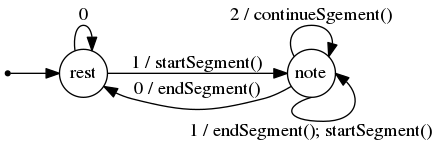
\includegraphics[scale=0.75]{resources/visualizationFSM}
    \caption{Visualization State Machine}
    \label{fig:visualizationStateMachine}
  \end{center}
\end{figure}

\begin{figure}
  \begin{center}
    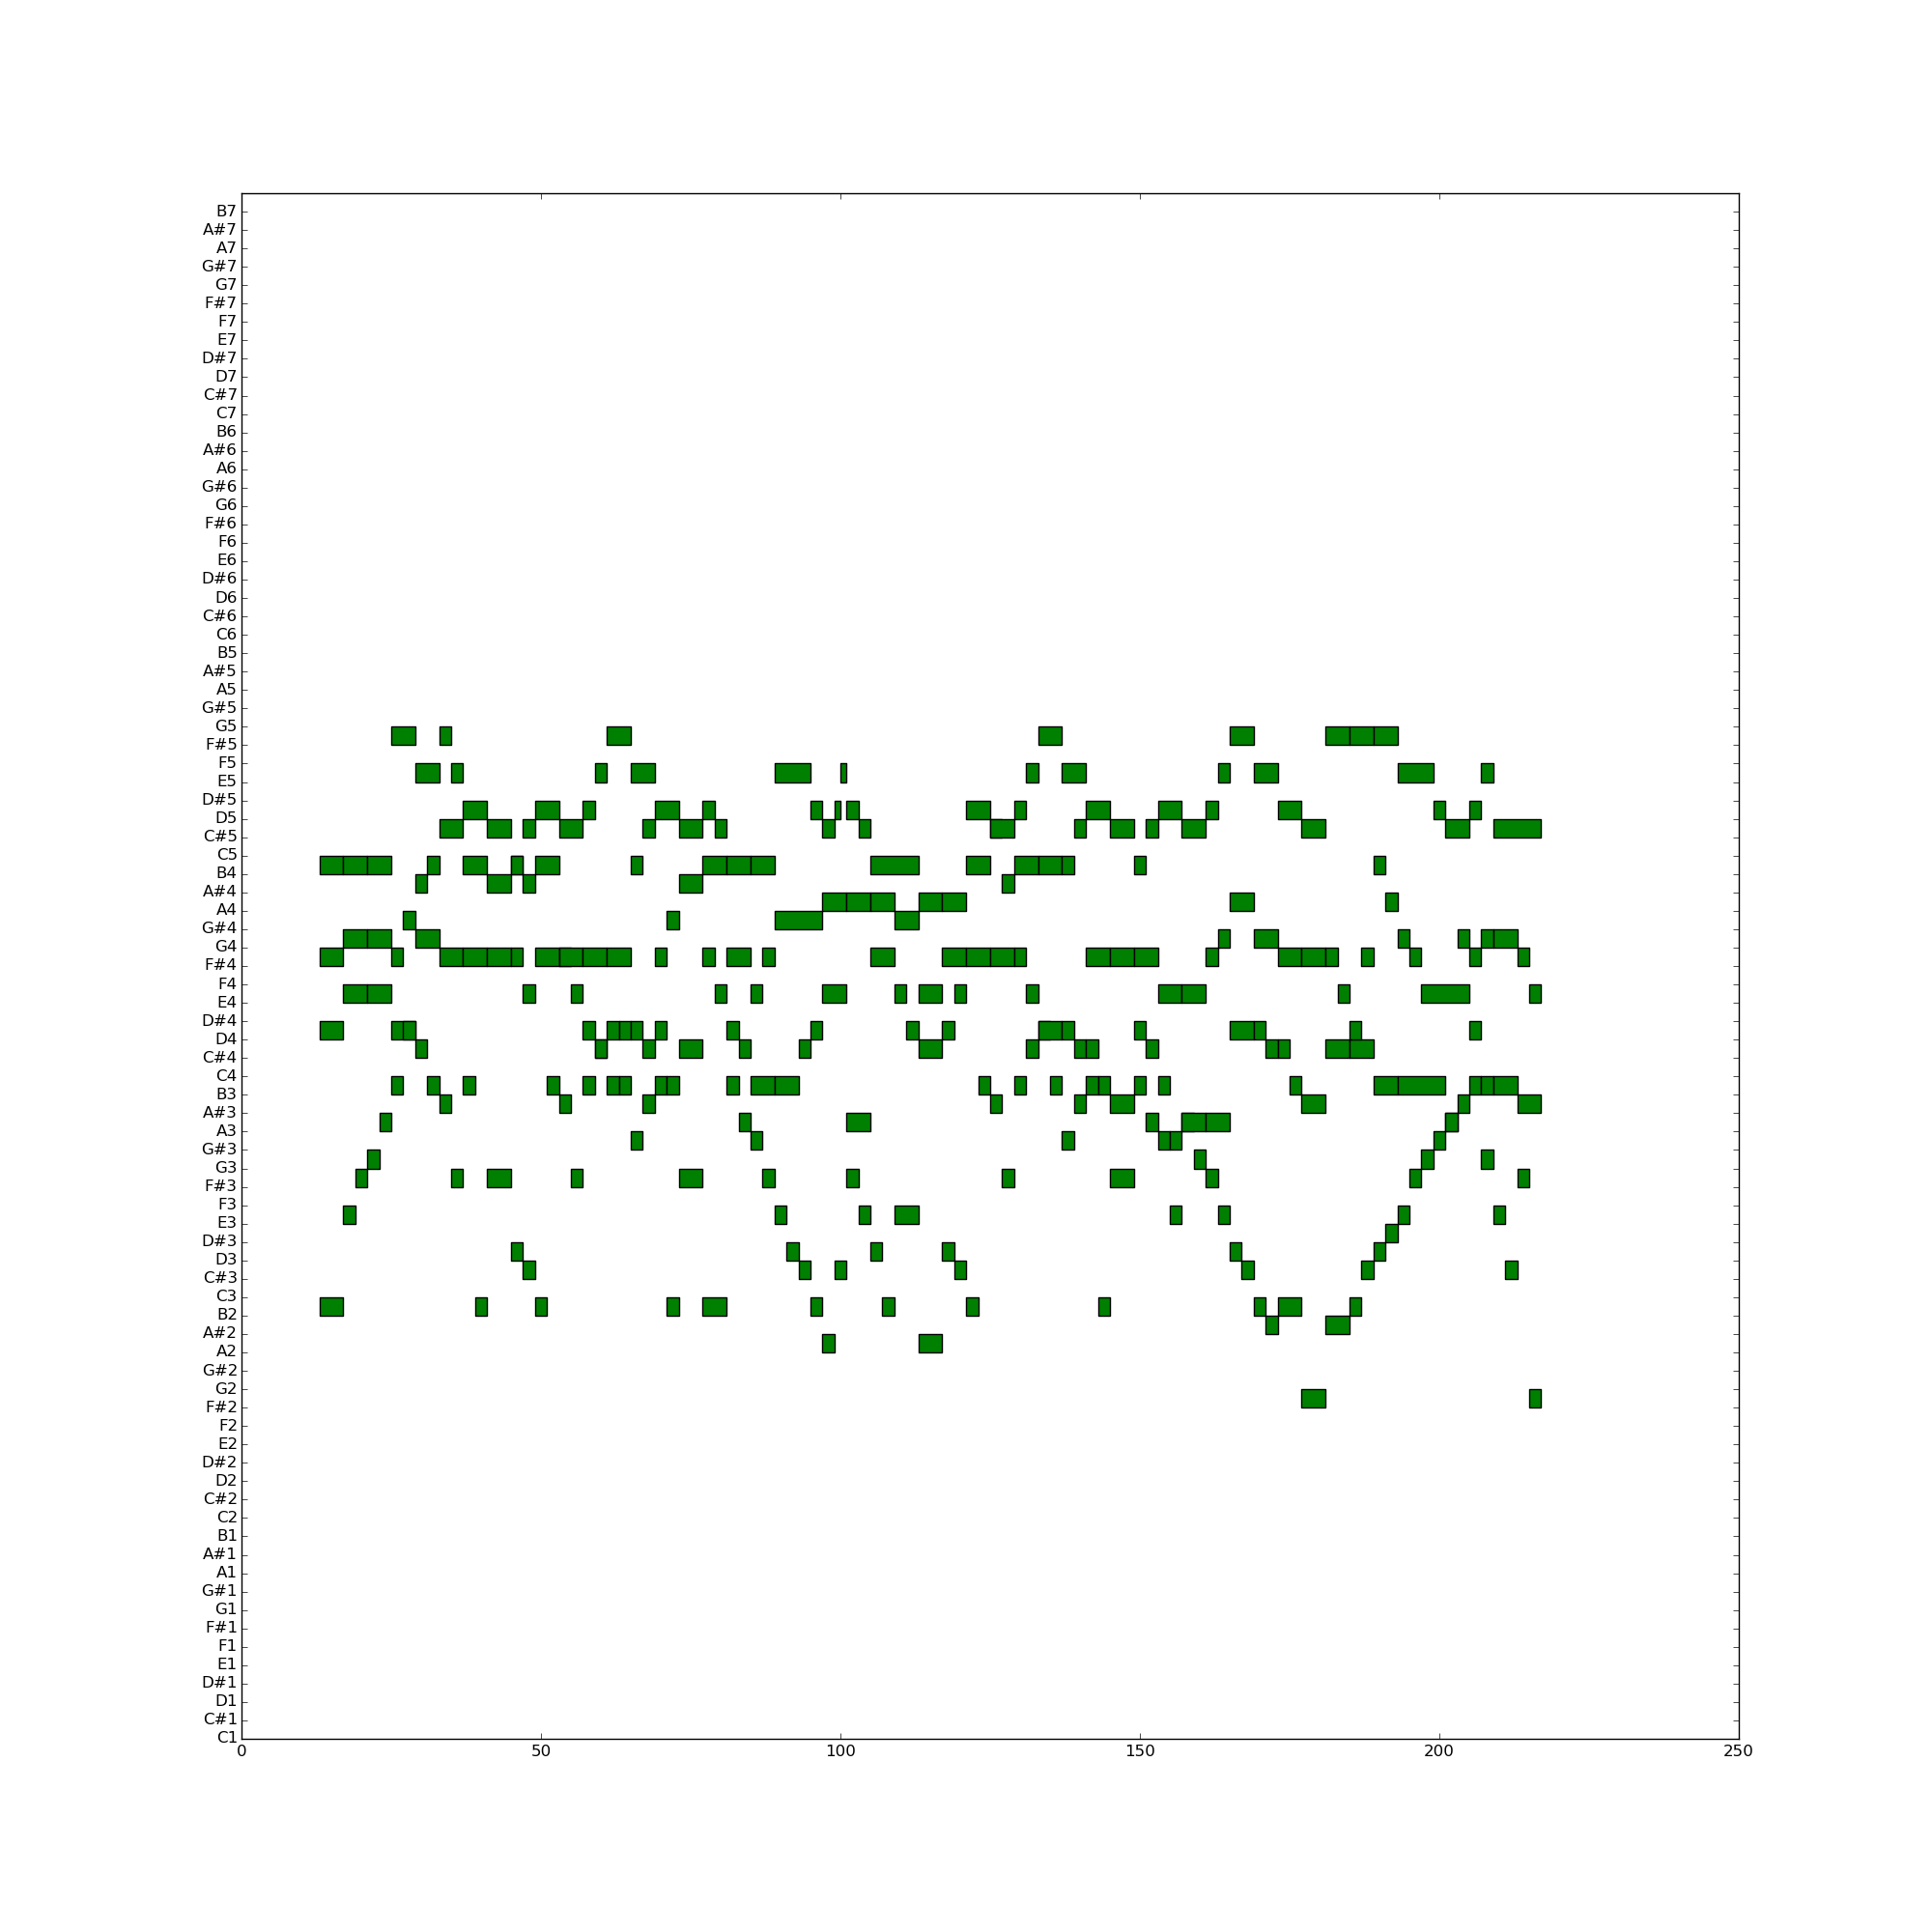
\includegraphics[scale=0.35]{resources/bwv108PianoRoll}
    \caption{Piano Roll Visualization of J.S. Bach BWV 108, Last Movement}
    \label{fig:bwv108PianoRoll}
  \end{center}
\end{figure}

\subsection{MIDI Visualization}

When creating a visualization directly from a MIDI file, the algorithm used depends on the type of MIDI file used. As described in ``Beyond MIDI'' \citep*{HeSe97}, there are three possible types of MIDI files; format 0, format 1, and format 2. Format 0 restricts data to a single track, format 1, allows multiple independent melodic tracks which are all synchronized to a single time line, and format 2 allows tracks which are temporally independent. When dealing with a format 0 or format 1 MIDI file, constructing the visualization is similar to visualizing a VMF file by plotting notes on the timeline by observing the note-on and note-off MIDI messages. When dealing with format 2 MIDI files, some additional work is necessary to synchronize all tracks to the same time line before plotting notes on the timeline.

\subsection{Humdrum Visualization}

When using a Humdrum file using the **kern format as as source for a piano roll visualization, a pre-processing step is necessary to achieve the same accuracy that VMF provides. In **kern, each pitch token is given a duration value. These duration values are equivalent to rhythmic durations seen in western music notation (ex. eighth note, sixteenth note, ...). To build the time axis of a piano roll visualization and plot notes, the largest common denominator of all the duration values to display must be determined to be used as the basic time unit. For example, if the music in \ref{fig:voicesExample} was encoded as a **kern Humdrum file, a pre-processing stage is required to determine that the eighth note is the greatest common denominator of all duration values in the piece to be visualized. Once this unit is determined, notes can be plotted by calculating how many duration units is necessary to represent each note's length accurately. In the case of the music in \ref{fig:voicesExample}, an eighth note requires one unit, a quarter note requires two units, and a half note requires four units.

By following this procedure, a **kern Humdrum file can be visualized, but the pre-processing step adds extra complexity which is not present when using a VMF file as a source.

\subsection{MusicXML Visualization}

Like VMF and MIDI, MusicXML encodes duration using a ``tick'' system where note durations are described in terms of subdivisions of a quarter note. In the simplest of cases, this lends itself well to piano roll visualization as in the case of VMF, however, MusicXML has some differences in this system which can cause complications when constructing a visualization of this nature. In polyphonic music, MusicXML allows different parts to use a ticks of a different value to describe note duration. For example, it is acceptable for one part to have a tick value of one third of a quarter note and another part to have a tick value of one half of a quarter note. In a case like this, it would be necessary to convert all parts to use a common tick value to facilitate visualization. Finally, MusicXML also allows the value of a tick to change in the middle of a part. Like the last case, the entire part would have to be converted to use a common tick value for the same reasons.

With any of the described formats, piano roll visualization is possible, but in some cases, varying degrees of pre-processing is necessary before the visualization can be constructed. VMF provides an advantage over these other formats as no pre-processing or computation is necessary to construct the visualization.
%!TEX root = vmf_main.tex

\section{Future Work}

Future work which is of interest for the VMF project includes designing and building a synthesizer which can playback music encoded in VMF. At the current time, if one wishes to play back the music contained in a VMF file, they must first convert the VMF file to a MIDI file using the converter described earlier in this paper and then playing back the file using any of the available MIDI sequencers.

If a synthesizer is implemented, the creation of a method to streamline input into VMF would also be of great use. As it stands, the only way to produce a VMF file is by converting an existing file from MIDI, Humdrum, MusicXML, or any other format currently supported by the music21 toolkit to VMF using the provided converter. An ideal adapter tool would be one which allows the use of a MIDI instrument such as a keyboard to be used to record directly to VMF.

Finally, to open VMF recording to the world outside of MIDI, investigating how to convert an audio signal to an appropriate VMF encoding for simple monophonic melodies would be of great value for information retrieval applications allowing a user to play a melody on their instrument or to hum a melody into a microphone to query a VMF database for the score which the melody belongs to or other similar scores.

The inclusion of a synthesizer and input adapters would definitely help to establish a robust toolkit surrounding VMF enabling more interesting applications featuring VMF to be created in the future.
\vspace*{24pt}

% %References
\bibliographystyle{cmj}
\bibliography{vmf_main}

\end{document}
